\documentclass[12pt]{standalone}
\usepackage[utf8]{inputenc}
\usepackage[T1]{fontenc}
\usepackage{times}
\usepackage{amsmath,amssymb}
\usepackage[dvipsnames,svgnames]{xcolor}
\usepackage{tikz}
\usetikzlibrary{calc, positioning, arrows.meta}
\definecolor{winblue}{HTML}{0D366B}
\definecolor{inksec}{HTML}{52514E}
% Adaptado de Marzetta et al. (2016), Fig. 1.4(a), p. 12: arranjo linear (ULA) no lugar do cilindro,
% "Equalization" no lugar de "Decoding".
\newcommand{\phone}[1]{%
  \begin{scope}[shift={#1}]
    \draw[line width=0.7pt, fill=black!20, rounded corners=1pt] (-0.13,-0.24) rectangle (0.13,0.24);
    \draw[line width=0.7pt] (0.06,0.24) -- (0.06,0.33);
  \end{scope}}
\newcommand{\antena}[1]{%
  \begin{scope}[shift={#1}]
    \draw[line width=0.8pt] (0,0) -- (0,0.18);
    \draw[line width=0.8pt] (0,0.18) -- (-0.1,0.32);
    \draw[line width=0.8pt] (0,0.18) -- (0.1,0.32);
  \end{scope}}
\begin{document}
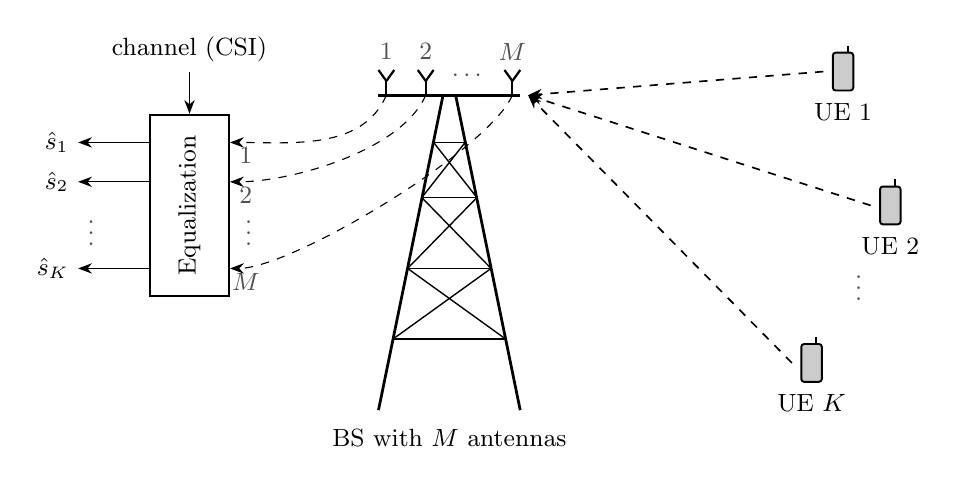
\begin{tikzpicture}[font=\fontsize{9}{10.8}\selectfont, >={Stealth[length=5pt]}]
% torre
\draw[line width=1pt] (-0.9,0) -- (-0.08,4.0);
\draw[line width=1pt] (0.9,0) -- (0.08,4.0);
\foreach \y/\h in {0.9/0.72, 1.8/0.53, 2.7/0.35, 3.4/0.2}
  \draw[line width=0.6pt] (-\h,\y) -- (\h,\y);
\draw[line width=0.5pt] (-0.72,0.9) -- (0.53,1.8) (0.72,0.9) -- (-0.53,1.8)
                        (-0.53,1.8) -- (0.35,2.7) (0.53,1.8) -- (-0.35,2.7)
                        (-0.35,2.7) -- (0.2,3.4) (0.35,2.7) -- (-0.2,3.4);
% arranjo linear de M antenas
\draw[line width=1pt] (-0.9,4.0) -- (0.9,4.0);
\foreach \x/\l in {-0.8/1, -0.3/2, 0.8/M} {
  \antena{(\x,4.0)}
  \node[inksec] at (\x,4.55) {$\l$};
}
\node[inksec] at (0.25,4.25) {$\cdots$};
\node[align=center] at (0,-0.35) {BS with $M$ antennas};
% bloco de equalizacao
\node[draw, line width=0.8pt, minimum width=1.0cm, minimum height=2.3cm] (eq) at (-3.3,2.6) {\rotatebox{90}{Equalization}};
\draw[->] (-3.3,4.3) node[above] {channel (CSI)} -- (eq.north);
\foreach \x/\y/\l in {-0.8/0.8/1, -0.3/0.3/2, 0.8/-0.8/M} {
  \draw[->, dashed] (\x,4.0) .. controls (\x-0.3,3.3) and (-2.0,2.6+\y) .. ($(eq.east)+(0,\y)$);
  \node[inksec] at ($(eq.east)+(0.2,\y-0.17)$) {$\l$};
}
\node[inksec] at (-2.55,2.35) {$\vdots$};
\foreach \y/\l in {0.8/1, 0.3/2, -0.8/K}
  \draw[->] ($(eq.west)+(0,\y)$) -- ++(-0.9,0) node[left] {$\hat s_{\l}$};
\node[inksec] at (-4.55,2.35) {$\vdots$};
% UEs
\foreach \x/\y/\l in {5.0/4.3/1, 5.6/2.6/2, 4.6/0.6/K} {
  \phone{(\x,\y)}
  \node[below] at (\x,\y-0.28) {UE $\l$};
  \draw[->, dashed, line width=0.6pt] (\x-0.25,\y) -- (1.0,4.0);
}
\node[inksec] at (5.2,1.65) {$\vdots$};
\end{tikzpicture}
\end{document}
